\documentclass[11pt]{article}
\usepackage{graphicx}
\usepackage[top=1in, bottom=1in, left=0.5in, right=0.5in]{geometry}
\begin{document}
\title{CS296 Group-8 Project: Virtual Rube Goldberg Machine}
\author{
		Janga Varun - 110050076\\\texttt{jangavarun@cse.iitb.ac.in} \and
		M Rajeev Kumar - 110050052\\\texttt{kumar@cse.iitb.ac.in} \and
		Shubham Mehta - 110050013\\\texttt{geniussm@cse.iitb.ac.in}
}

\date{\today}
\bibliographystyle{plain}
\maketitle

\section{Introduction}
This report describes the final submission of our Virtual Rube Goldberg Machine \cite{ru} which we have made using Box2D \cite{box}Library of c++. To start with we saw some videos of rube goldberg machine simulation on you tube \cite{vid1} \cite{vid2}.
The report begins with our decision to change the original design, so as to make things more feasible. 
Next it tries to answer the question-"What is so special about Our Machine?". After describing the pecularities of our design for a while, it turns to the deeper section, i.e. The Analysis of Code. For analysing code we have made different timing graphs using matplotlib \cite{pydoc} of python \cite{pyhelp} and also we have compared two situations, one having low load and other higgh load. There after it goes about the profiler data we received from perf and as to how we optimized our code from that. In the end, we try to conclude the report with references \cite{wi} \cite{km}.
\newpage

\section{Deviation from initial design}
\begin{center}
 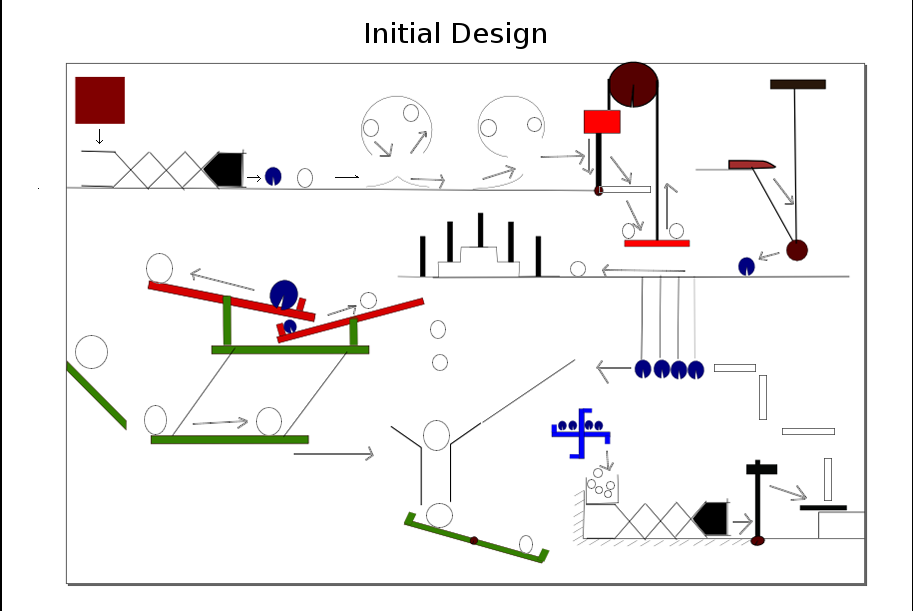
\includegraphics[width=0.8\textwidth,keepaspectratio]{img/design_directions.png}\\
 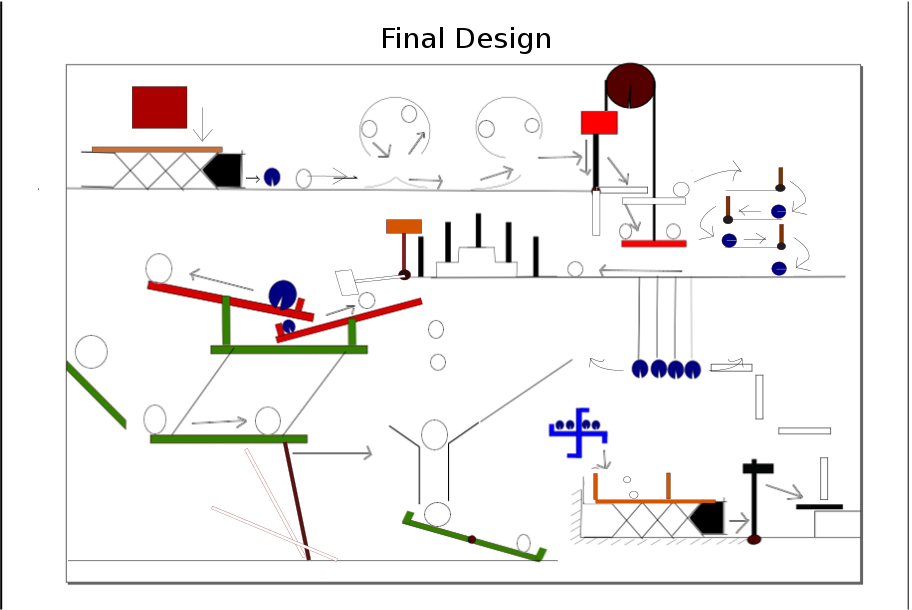
\includegraphics[width=0.8\textwidth,keepaspectratio]{img/design_new_directions.png}
\end{center}

\subsection{New plank above the Spring}
\begin{center}
 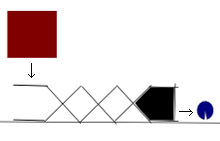
\includegraphics[width=0.3\textwidth,keepaspectratio]{img/spring_old.png}
 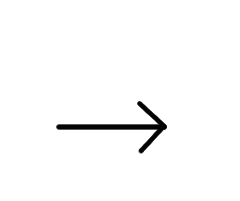
\includegraphics[width=0.3\textwidth,keepaspectratio]{img/arrow.png}
 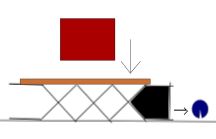
\includegraphics[width=0.3\textwidth,keepaspectratio]{img/spring_new.png}
\end{center}
	In the first part, the spring was bouncing at the right end up due to some torque and the normal force from the ground.
	So, a plank has been kept for having uniform distribution of force.

\subsection{Knife System replaced with Ball-Rotating Plank System}
\begin{center}
 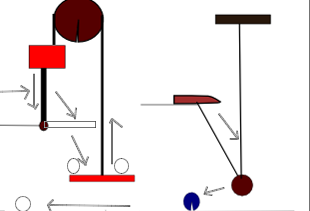
\includegraphics[width=0.3\textwidth,keepaspectratio]{img/knief.png}
 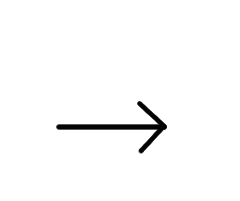
\includegraphics[width=0.3\textwidth,keepaspectratio]{img/arrow.png}
 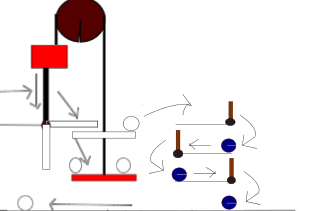
\includegraphics[width=0.3\textwidth,keepaspectratio]{img/rot_ball_plank.png}
\end{center}
	In the Box2D Documentation Manual we haven't found any Object which can cut/remove threads.
	So, we have implemented Balls-Rotating Planks System as a replacement to it, which does the same thing.
	Also this is more pleasing to eyes than the sharp knife.

\subsection{Hammer after the dominos}
\begin{center}
 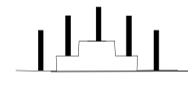
\includegraphics[width=0.3\textwidth,keepaspectratio]{img/dominos.png}
 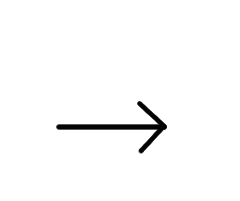
\includegraphics[width=0.3\textwidth,keepaspectratio]{img/arrow.png}
 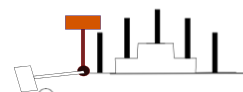
\includegraphics[width=0.3\textwidth,keepaspectratio]{img/dominos_with_hammer.png}
\end{center}
Without the hammer, the last domino falls into the funnel which disturbs the initial plan,
so an additional hammer is created which actually manages the fall of the balls in a smart way
(When the small ball hits the hammer, it rebounds and that time is used for the Big ball to fall off).
Also the hammer is used to keep the rod still for some time, which assures the falling of the small ball in the funnel.

\subsection{Introduced a rod below the oscillating plank}
\begin{center}
 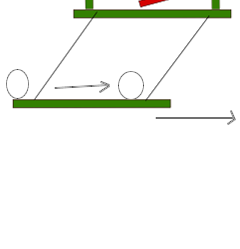
\includegraphics[width=0.3\textwidth,keepaspectratio]{img/without_rod.png}
 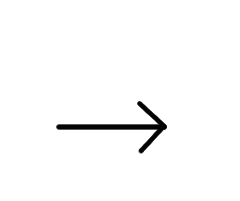
\includegraphics[width=0.3\textwidth,keepaspectratio]{img/arrow.png}
 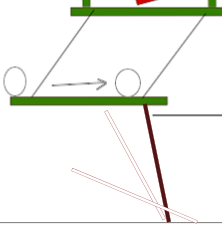
\includegraphics[width=0.3\textwidth,keepaspectratio]{img/with_rod.png}
\end{center}
	The problem was that we had to vary densities and frictions of the oscillating bars, inclined plank and the big ball to get a go to make the ball land on the swing as it reaches the right end of the plank. Also the code doesnt work same way in all platforms.
	Without using a rod below the oscillating plank, it has been too time 
	consuming for seeing that the code works on both 32-bit and 64-bit machines.
	So, we have set a rod which falls just after the big ball falls on the oscillating plank.

\section{What makes our design interesting?}
\subsection{Spring system}
\begin{center}
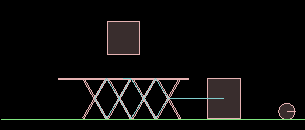
\includegraphics[width=0.4\textwidth,height=0.1\textheight]{img/spring1} 
\hspace{3em}
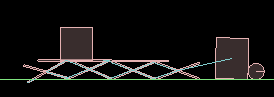
\includegraphics[width=0.4\textwidth,height=0.1\textheight]{img/spring2}
\end{center}
When the heavy box falls on the spring system, the spring compresses almost always parallel to the ground. This is due to the rod present on the spring which spreads the force equally across the whole area.

\subsection{Circular paths}
\begin{center}
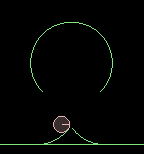
\includegraphics[width=0.2\textwidth,height=0.2\textheight]{img/circle1} 
\hspace{6em}
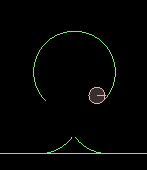
\includegraphics[width=0.2\textwidth,height=0.2\textheight]{img/circle2}
\end{center}
The ball, after hit by the punching box, rushes from the ramp trying to traverse a circle in the path above the ramp.
The interesting thing to note here is the accuracy in ball's position, when it reaches the circular path.

\subsection{Pulley System}
\begin{center}
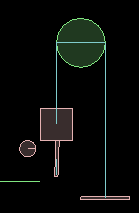
\includegraphics[width=0.2\textwidth,height=0.2\textheight]{img/pulley1} 
\hspace{2em}
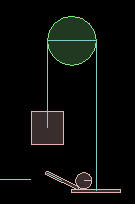
\includegraphics[width=0.2\textwidth,height=0.2\textheight]{img/pulley2}
\hspace{2em}
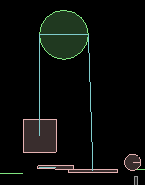
\includegraphics[width=0.2\textwidth,height=0.2\textheight]{img/pulley3}
\end{center}
The ball, after traversing 1.75 circular paths, hits the rod kept as a support to the box attached to the pulley.
This makes the box to fall and the plank on the other side rises. After that, the rod itself and the plank form a bridge for the ball. The ball travels on the bridge and finally gets to the other side. The interesting thing here is the synchronization of the ball, rod, box and the plank. If any one of them is a bit denser or shorter, the box would not be able to cross.

\subsection{Hammer, balls and the rotating bars}
\begin{center}
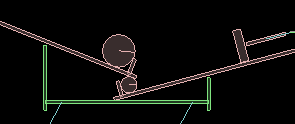
\includegraphics[width=0.25\textwidth,height=0.1\textheight]{img/hammer1} 
\hspace{2em}
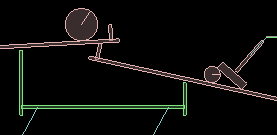
\includegraphics[width=0.25\textwidth,height=0.1\textheight]{img/hammer2}
\hspace{2em}
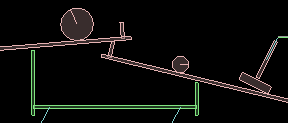
\includegraphics[width=0.25\textwidth,height=0.1\textheight]{img/hammer3}
\hspace{2em}
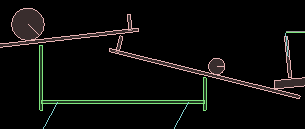
\includegraphics[width=0.25\textwidth,height=0.1\textheight]{img/hammer4}
\hspace{2em}
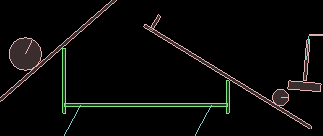
\includegraphics[width=0.25\textwidth,height=0.1\textheight]{img/hammer5}
\end{center}
Here the small ball is a bouncing ball. Firstly the hammer hits on the right rod and this makes the two abrs along with the balls to raise and stay still there after. As the mass is less, the smaller ball starts to move first and hits the hammer and bounces back. While this ball moves back, the bigger ball moves on towards the hinge of the left bar. By the time the bigger ball crosses the hinge, the small ball is moving towards the hammer, and then the bigger ball moves a little bit more making the left bar lift even higher, making the right bar lift too. This lifting provides the small ball a small opening to go forward and fall in the funnel. Here many factors had to be varied to get a good sync.

\subsection{Swing and the big ball}
\begin{center}
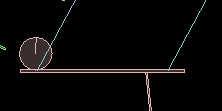
\includegraphics[width=0.2\textwidth,height=0.1\textheight]{img/swing1} 
\hspace{2em}
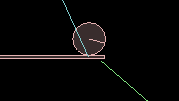
\includegraphics[width=0.2\textwidth,height=0.1\textheight]{img/swing2}
\end{center}
As the small ball falls into the funnel and tries to rest on the see-saw, the bigger ball falls on the inclined plank and reaches the left end of the swing, just supported by a rod from below. The swing sets loose as soon as this happens. The bigger ball reaches the right end of the swing as the swing reaches the funnel. The bottom rod's and the inclined plank's inclination had to be varied many times to get exact sync.

\subsection{Hammer, rod and the 4 balls}
\begin{center}
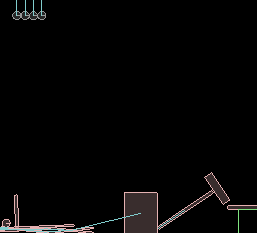
\includegraphics[width=0.2\textwidth,height=0.2\textheight]{img/osc1} 
\hspace{2em}
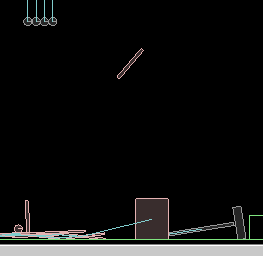
\includegraphics[width=0.2\textwidth,height=0.2\textheight]{img/osc2}
\hspace{2em}
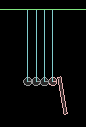
\includegraphics[width=0.2\textwidth,height=0.2\textheight]{img/osc3}
\end{center}
The end hammer is touched by the second punching box when the smaller balls fall in the basket attached to the spring system. Then the hammer falls on the rod lying on the corner of a step. The rod rises rotating in the air and hits the last ball attached on the top. This process is made as much as in synch as possible by varying the hammer's and rod's density.

\subsection{Works in both 32 and 64 bit Ubuntu Platforms}
As the title says, our simulation works in both the platforms. It is very important for us to state this as we have spent a lot of time in maintaining the sync in both platforms. We have learnt that Box2d is not deterministic and is compiler and processor dependent. So we tried to make the simulation run in both platforms with as less differences as possible.


\section{Analysis of Code}
\subsection{Graph 1}
 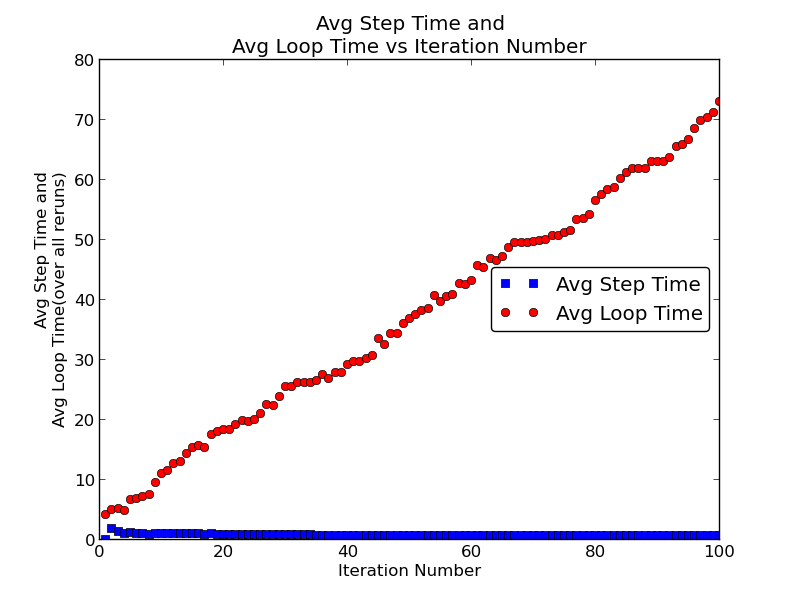
\includegraphics[width=0.5\textwidth,keepaspectratio]{img/g08_plot01_low} 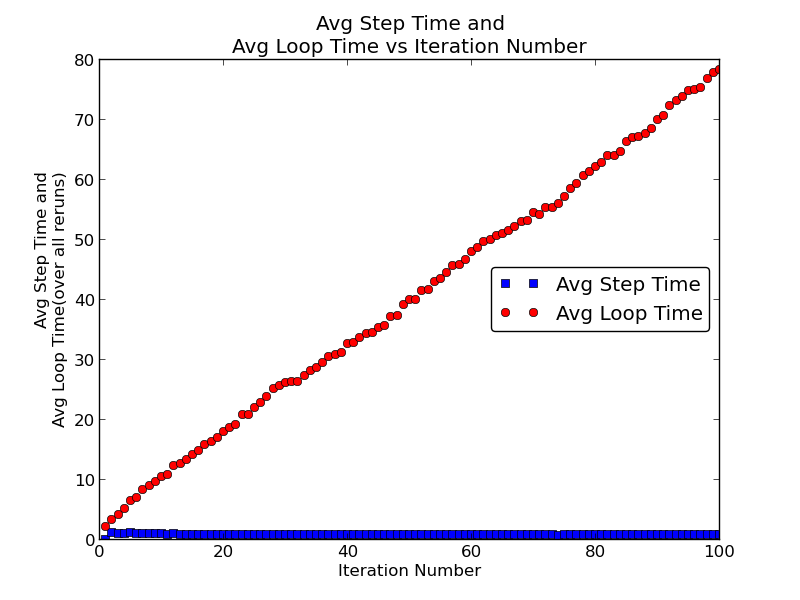
\includegraphics[width=0.5\textwidth,keepaspectratio]{img/g08_plot01_high}
In Graph 01 we have plotted Average Step Time Values and Average Loop time values against Iteration Value. The graph is decreasing in average step time which implies that initial steps were consuming more time than further steps.  The Average loop time is incresing with number of iterations as with iteration number total calculation also increases. Also there is no sharp edge or any disorder in graph at any iteration value because in initial 100 steps ball-1 reaches almost the top of first cicular loop so the collisions happening and velocity claculations included in these steps are almost the same in each of them.\\
On repeating the same experiment with higher load the average loop time increases for all iterations because of less RAM available for execution of code. Though the overall pattern of the graphs in both the cases are almost the same.\\

\subsection{Graph 2}
 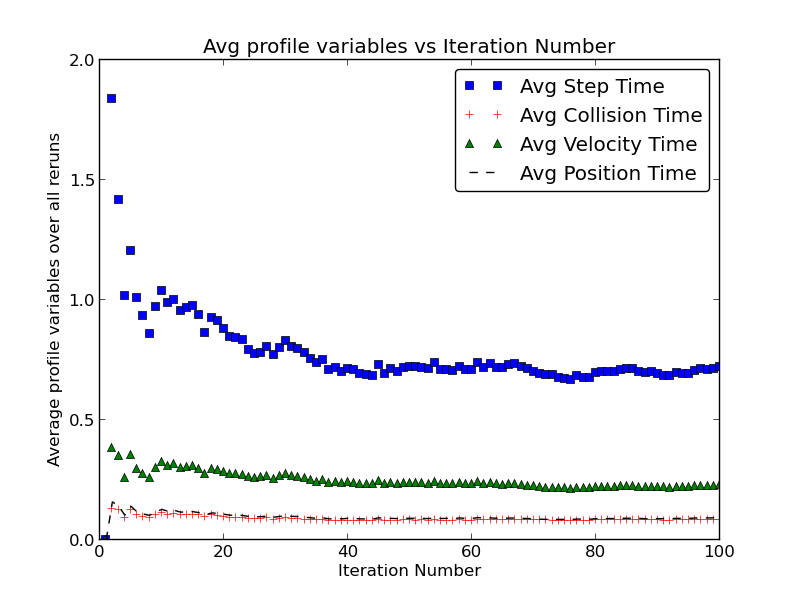
\includegraphics[width=0.5\textwidth,keepaspectratio]{img/g08_plot02_low} 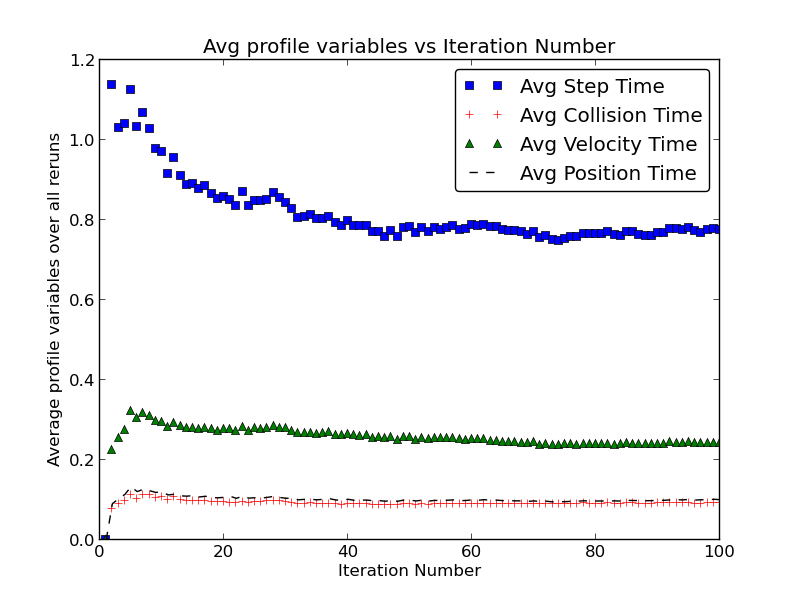
\includegraphics[width=0.5\textwidth,keepaspectratio]{img/g08_plot02_high}
In Graph 02 we have plotted avg step time , avg collison time , avg. velocity time, avg. collison time, avg. position time against no. of iterations.
Like we saw in graph 01 avg. step time decreases with no. of steps which implies that time taken for step decraeses with step number.\\
Collison Time : time for which the collison lasts and also to check if any collison has happened.\\
Velocity Update Time: time to update velocity of all objects at each step.\\
Avg. Position Time: Time to calculate positions of different Box 2D objects present.\\ 
The average collision detection time, velocity update time and position update time remains almost constant because the number of solid objects are constant. They are constant because they only depend on number of steps in simulation and are also proportional to number of objects and in calculation we have averaged them with the iteration value i.e. number of steps.
On repeating the same experiment with higher load the average loop time increase for all iterations because of less RAM available for execution of code.Although, the pattern of all the plots is the same in both the cases.\\

\subsection{Graph 3}
 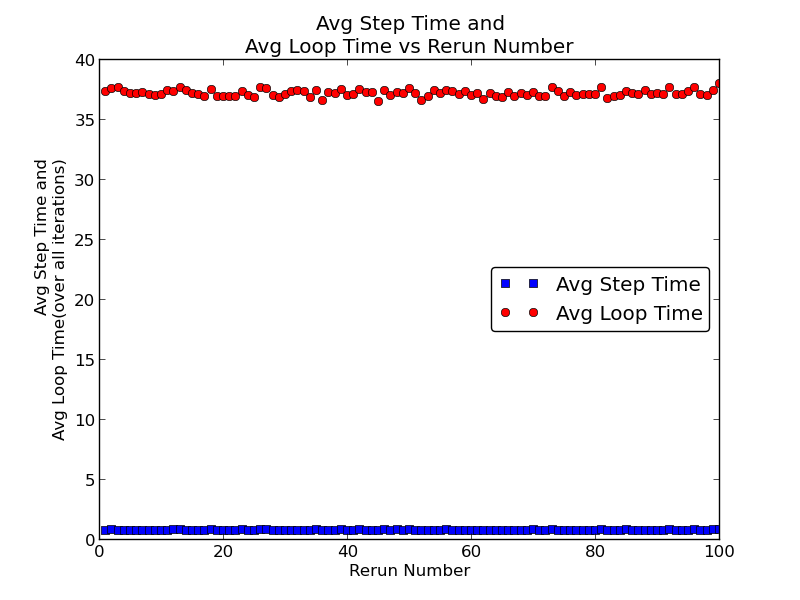
\includegraphics[width=0.5\textwidth,keepaspectratio]{img/g08_plot03_1_low} 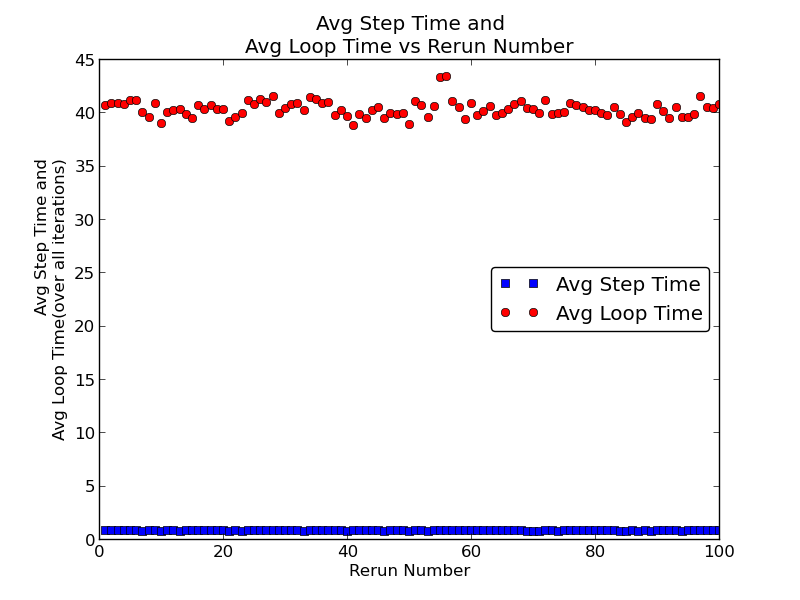
\includegraphics[width=0.5\textwidth,keepaspectratio]{img/g08_plot03_1_high}
In Graph 03 we have plotted average step time values and total loop time value over all iterations against the rerun value.\\
Both the graphs are coming almost constant with respect to avg. loop time and avg. step time because time only depends on iteration number and not on rerun number so when we take avg. of times over iteration numbers crreponding to different rerun numbers it stays almost constant.\\  
But when we increase the load it increases the time values according to the load although it is also almost constant but there are deflections in points plotted in case of high load graph as I used youtube videos to increase load and they vary their RAM uses with time.\\

\subsection{Graph 4}
 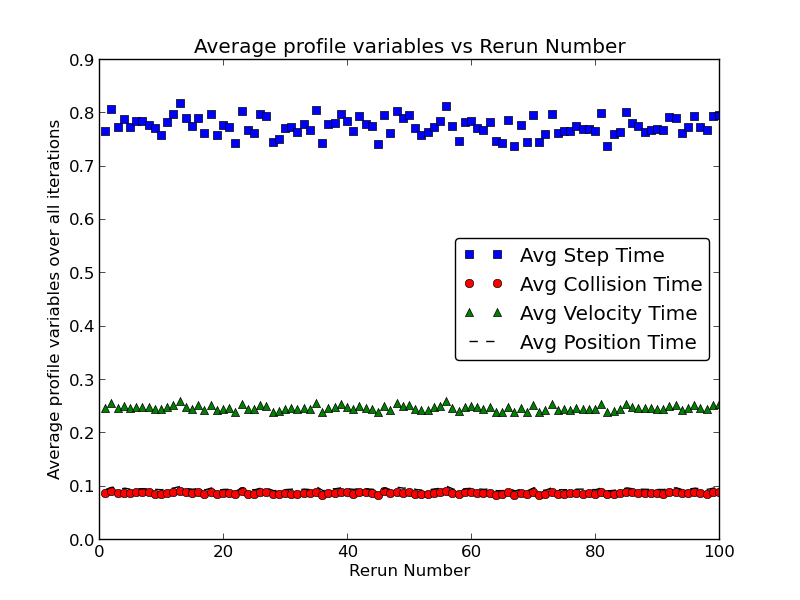
\includegraphics[width=0.5\textwidth,keepaspectratio]{img/g08_plot03_low} 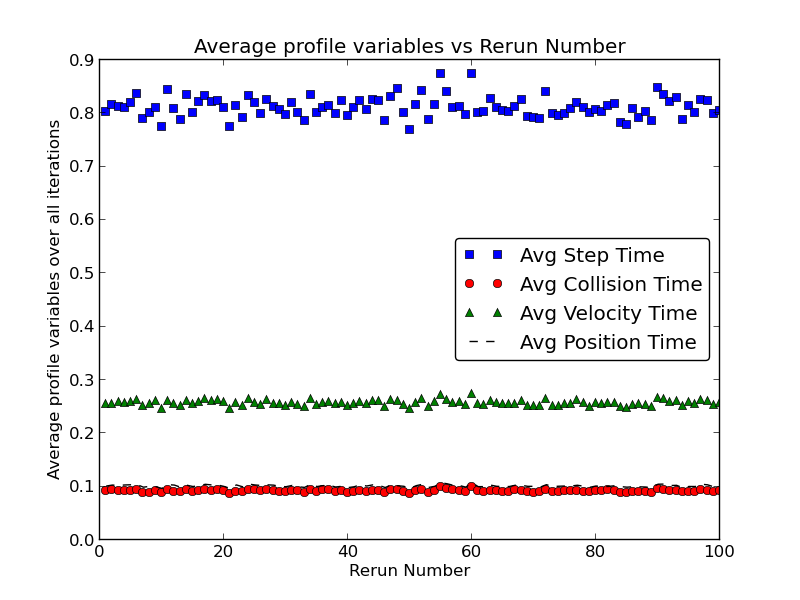
\includegraphics[width=0.5\textwidth,keepaspectratio]{img/g08_plot03_high}
In Graph 04 we have step times, collision detection times, velocity update times and position update times averaged over all iterations against rerun number of graph.\\
All the values are coming constant with respect to the number of rerun since as mentioned above time of program only depends on iteration value i.e. number of steps and in this case we have averaged it over all iteration values for different rerun values, so values are constant only depending on RAM condition at which rerun is performed.\\
So when we increase the load it increases the time values according to the load and otherwise it is almost constant.\\

\subsection{Graph 5}
 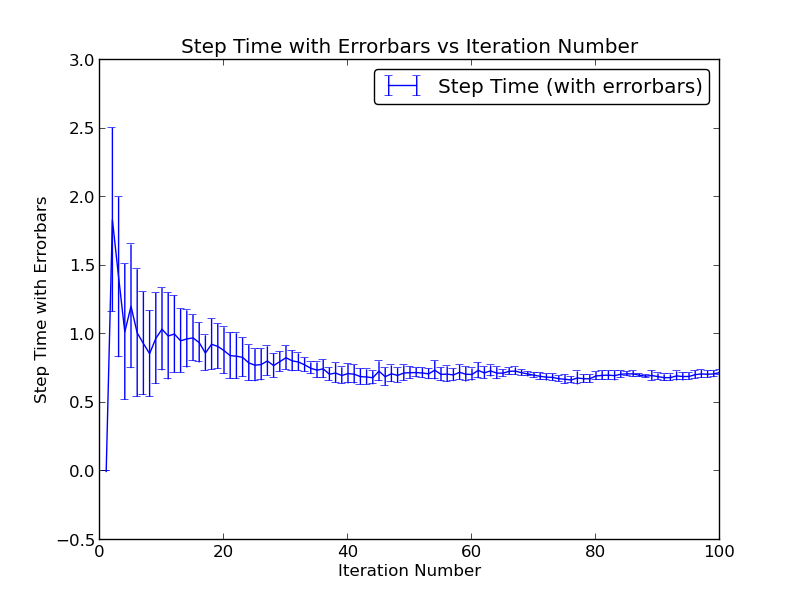
\includegraphics[width=0.5\textwidth,keepaspectratio]{img/g08_plot04_low} 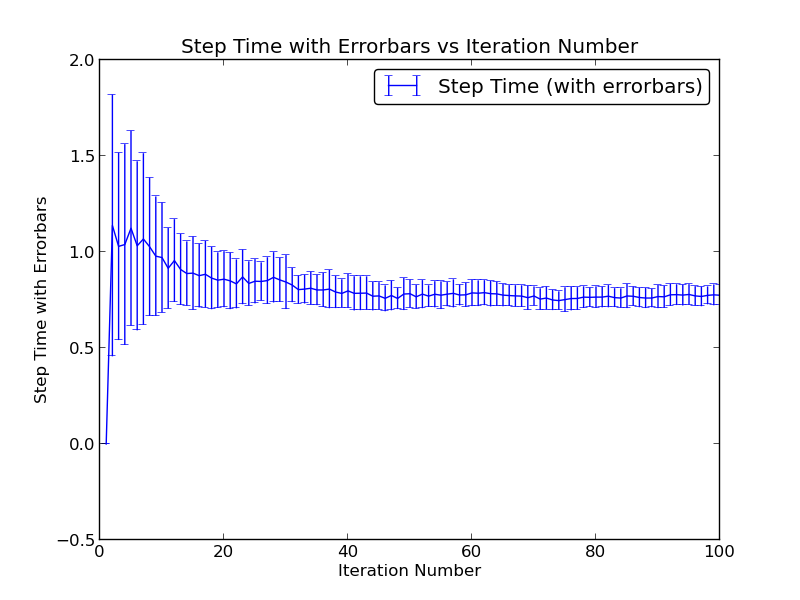
\includegraphics[width=0.5\textwidth,keepaspectratio]{img/g08_plot04_high}
In Graph 05 we have plotted step time values with error bars averaging them over different reruns against Iteration value.\\
For plotting error bars I have used standard deviation for a particular iteration value for different rerun values. It appears from the graph that with increase in number of steps error value decreases slightly as for lesser number of steps deviation due to other process going on is more as compared to higher number of steps.\\
Also with increase in load tendency of step time to deviate from its average value also increases as fluctuations in other processes also induce error in execution of our code.\\

\subsection{Graph 6}
 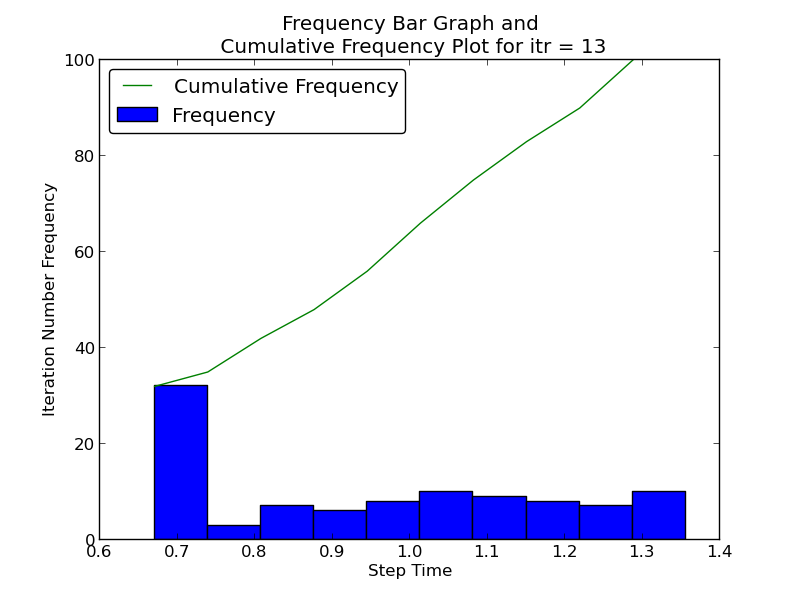
\includegraphics[width=0.5\textwidth,keepaspectratio]{img/g08_plot05_low} 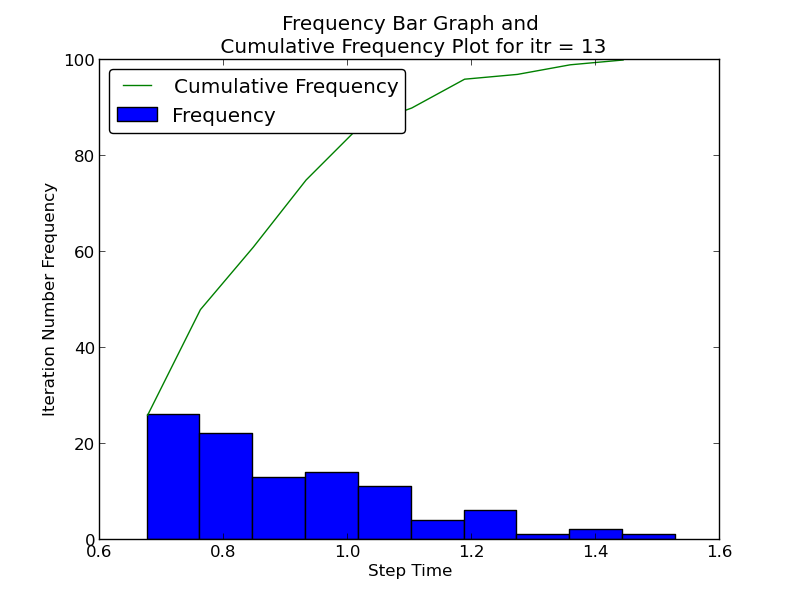
\includegraphics[width=0.5\textwidth,keepaspectratio]{img/g08_plot05_high}
In Graph 06 I have plotted for a given iteration value (= 13) frequency and cumulative frequency of rerun numbers with respect to step time.\\
The graph has almost all the values concentrated in an area only few of them are flactuated which suggests the fact that for a iteration value time remains almost constant for differet reruns.\\
With increased load the distribution of rerun over step time increases i.e. error increases but most of reruns occur in same range of step time. This happens because fluctuation in load induces fluctuations in execution of our code.\\

\section{Comparison of Time and Gettimeofday}
Value obtained by time function is more than the value obtained by gettimeofday function because gettimeofday function includes only the time required for completion of ``for'' loop while Time function also includes the time required for starting execution of code and initialisation of variables alongwith
time required for completion of ``for'' loop.

\newpage
\section{Profilers}
We have used ``perf'' \cite{perf} \cite{prof} to profile our code. There are two versions of the code:\\
1) Debug Version \\
2) Release Version \\
The iteration value is taken as 10,000 so as to record the least called function also.
Also the caller-callee graph for the release version is mostly occupied with perf-related-functions for low iteration value. Another reason is that for lower iteration values, the release version has only one or two optimizable functions.

\subsection{Debug Version}
Debug Version is formed by using ``-DCMAKE\textunderscore BUILD\textunderscore TYPE=Debug'' flag while compiling the Box2D library and by removing any optimization flags while compiling the object files.\\
This code has all the debug symbols appended for future use.
So Debug code is almost the same as the original code.

\subsection{Release Version}
Debug Version is formed by using ``-DCMAKE\textunderscore BUILD\textunderscore TYPE=Release'' flag while compiling the Box2D library and by keeping optimization flags like -O2 or -O3 while compiling the object files.\\
This code is optimized as much as possible, due to which the executable runs faster.

\subsection{Debug vs Release}
\begin{enumerate}
\item Firstly the number of samples found in profiling release version is almost quarter of that found in debug version. This explains the level of optimization done by -O3 flag.\\
\item The use of optimization flags majorly causes the following:
\begin{itemize}
\item function inlining - \\
 replacing the function with its definition 
\item instruction scheduling - \\
 rearranging the order of instructions in order to avoid delays in execution
\item loop expansion - \\
 all the switch, for, while loops are unwinded 
\end{itemize}
\item The major functions optimized in the release profile:
\begin{itemize}
\item \textit{b2Vec2::b2Vec2(float, float)} - \\
 It is optimized using function inlining.
\item \textit{b2Cross(float, b2Vec2 const\&)}
\item all operator overloading functions
\end{itemize}

\item Also interestingly, sinf, cosf functions are converted to a single function sincosf in the math library.\\
\end{enumerate}

\subsection{Optimizable Code}
The top function in both the debug and release versions' profiles is 
\textit{b2ContactSolver::SolveVelocityConstraints()}

This function's overhead is also increased due to the relative decrease of overheads of other elementary and operator overloading functions.\\
But this function can be optimized. We can observe that ``vc$\rightarrow$points'', ``vcp$\rightarrow$tangentImpulse'' etc are used repeatedly which can be avoided by declaring a variable outside the loop.\\
Also variables such as ``b2ContactVelocityConstraint* vc'', ``b2Vec2 dv'' etc are declared repeatedly in every iteration, which causes reallocation of memory which is unwanted. This issue can be solved by declaring only once outside the loop.

\subsection{Call Graph} 
The number of blocks are reduced and
each block also has a color code according to its percentage.\\
Let the call graph have the following relation between A,B,C functions. A$\rightarrow$B$\rightarrow$C \\
If B is inline substituted, then the relation is changed to A$\rightarrow$C in the release graph.\\
e.g \\
b2ContactManager::Collide()
$\rightarrow$
b2Contact::Update(b2ContactListener*)
$\rightarrow$
b2PolygonAndCircleContact::Evaluate(b2Manifold*, b2Transform const\&, b2Transform const\&)
$\rightarrow$
b2CollidePolygonAndCircle(b2Manifold*, b2PolygonShape const*, b2Transform const\&, b2CircleShape const*, b2Transform const\&)
$\rightarrow$
operator-(b2Vec2 const\&, b2Vec2 const\&)

is changed to:\\
b2ContactManager::Collide()
$\rightarrow$
operator-(b2Vec2 const\&, b2Vec2 const\&)\\ \\

Call Graph for Release Version:\\
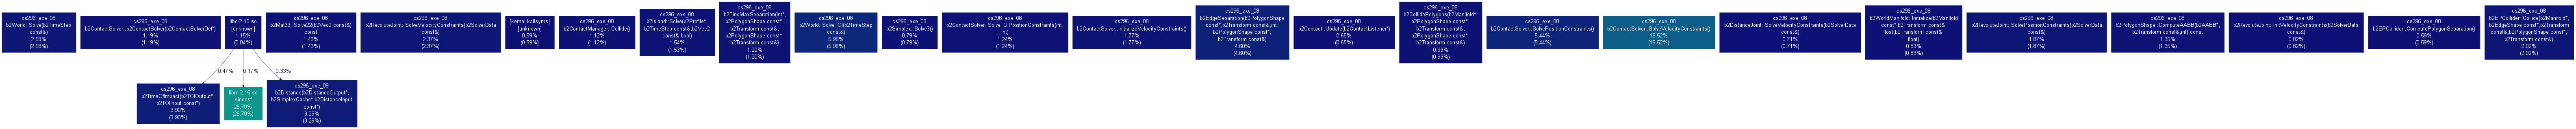
\includegraphics[width=1.0\textwidth,keepaspectratio]{img/g08_release}\\ \\ 
Call Graph for Debug Version:\\
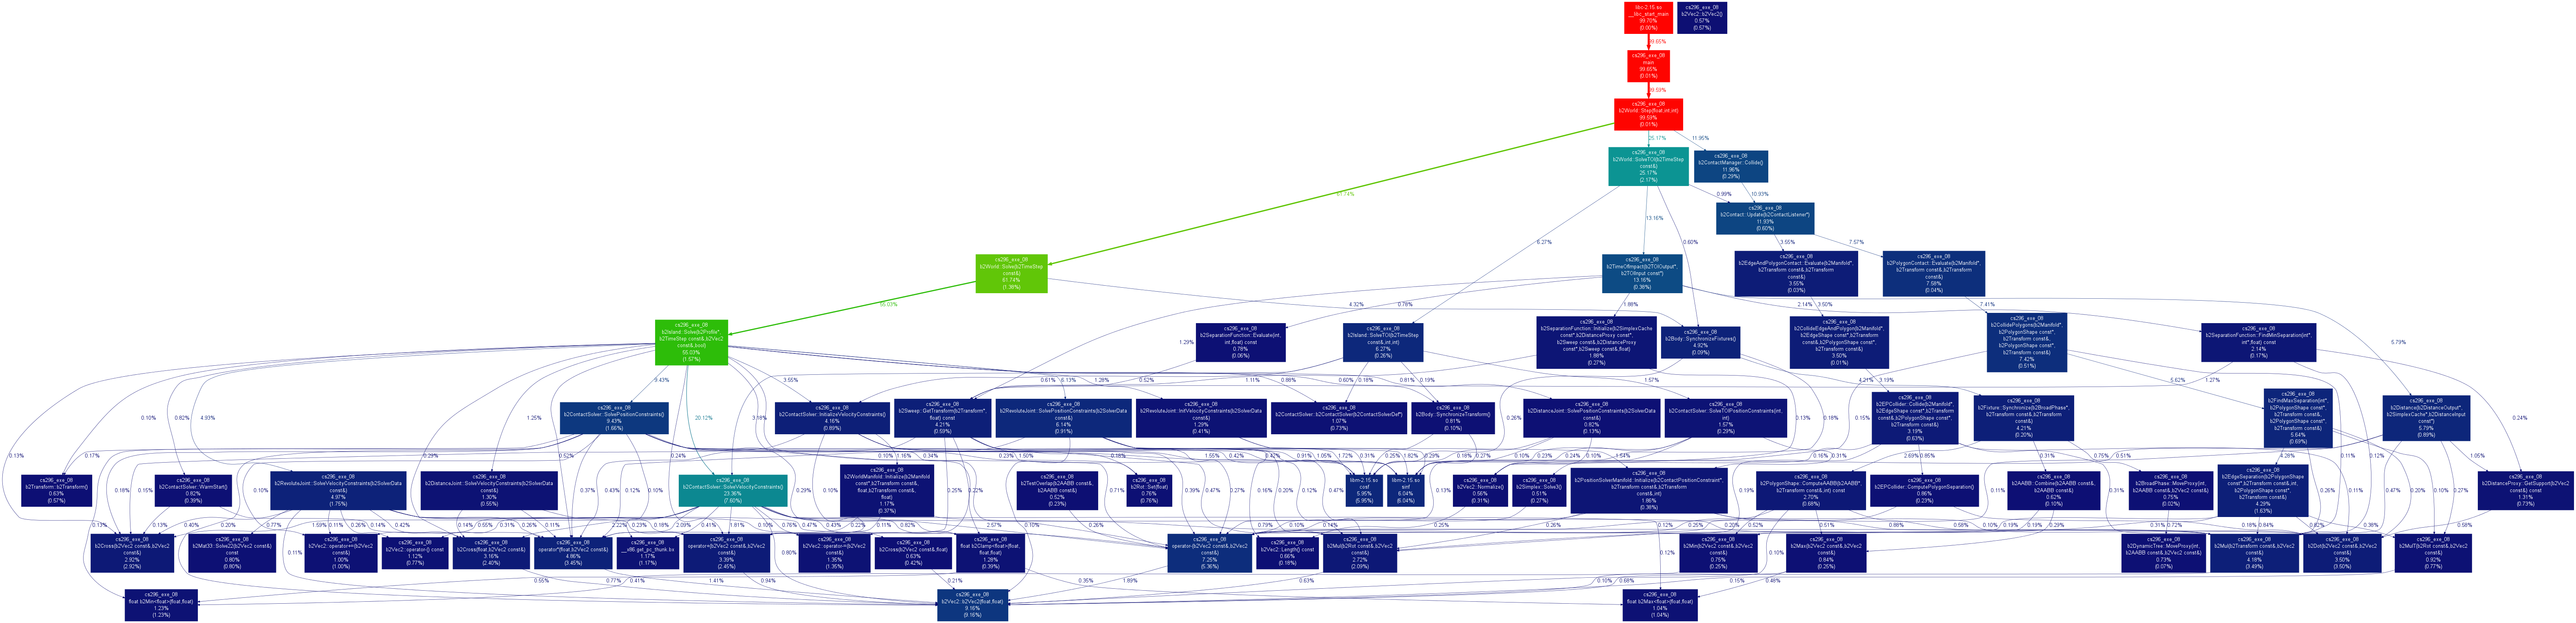
\includegraphics[width=1.0\textwidth,keepaspectratio]{img/g08_debug}
\bibliography{ref}
\end{document}
